\documentclass{UoNMCHA}
\usepackage[authoryear]{natbib}
\usepackage{array,booktabs} % For nice tables
\usepackage{amsmath,amsfonts,amssymb} % For nice maths
\usepackage{float}
\usepackage{color}
\usepackage{multicol}
\usepackage{enumerate}
\usepackage{listings}
\usepackage{subfig}
\usepackage{hyperref}
\usepackage[parfill]{parskip}   % For replacing paragraph indenting with a newline instead
\newif\ifcomment
\commenttrue
\commentfalse
% Number equations per section
\numberwithin{equation}{section}

\hypersetup{
%    bookmarks=true,         % show bookmarks bar?
%    unicode=false,          % non-Latin characters in AcrobatÕs bookmarks
%    pdftoolbar=true,        % show AcrobatÕs toolbar?
%    pdfmenubar=true,        % show AcrobatÕs menu?
%    pdffitwindow=false,     % window fit to page when opened
%    pdfstartview={FitH},    % fits the width of the page to the window
%    pdftitle={My title},    % title
%    pdfauthor={Author},     % author
%    pdfsubject={Subject},   % subject of the document
%    pdfcreator={Creator},   % creator of the document
%    pdfproducer={Producer}, % producer of the document
%    pdfkeywords={keyword1} {key2} {key3}, % list of keywords
%    pdfnewwindow=true,      % links in new window
    colorlinks=true,       % false: boxed links; true: colored links
    linkcolor=blue,          % color of internal links
    citecolor=blue,        % color of links to bibliography
%    filecolor=magenta,      % color of file links
    urlcolor=blue           % color of external links
}

\definecolor{light-gray}{gray}{0.95}
\definecolor{myblue}{RGB}{20,105,176}
\definecolor{myorange}{RGB}{255,140,0}
\definecolor{mygrey}{RGB}{64,64,64}
\definecolor{MATLABKeyword}{rgb}{0,0,1}
\definecolor{MATLABComment}{rgb}{0.1328125,0.54296875,0.1328125}
\definecolor{MATLABString}{rgb}{0.625,0.125,0.9375}

\lstset{language=Matlab,
    basicstyle=\small\ttfamily,
    keywordstyle=\color{MATLABKeyword},
    %identifierstyle=,
    commentstyle=\color{MATLABComment},
    stringstyle=\color{MATLABString},
    numberstyle=\tiny,
    %numbers=left,
    basewidth=0.5em}
\lstset{
language=C,
numbers=none,
xleftmargin=1cm,
frame=tblr,
classoffset=0,
morekeywords={LED_BUILTIN,HIGH,LOW,OUTPUT,INPUT,INPUT_PULLUP},keywordstyle=\color{myblue},
classoffset=1,
morekeywords={analogWrite,pinMode,write,Serial,begin,print,println,digitalWrite,delay,Stepper,step,setSpeed},	keywordstyle=\color{myorange},
classoffset=0,
commentstyle=\color{mygrey},
breaklines=true,
postbreak=\space //...
}

\firstpage{1}    % Set page number for first page
\UoNMCHAreportNo{ELEC1710  } %Report number
\UoNMCHAyear{ }   % Year
\shorttitle{ELEC1710 - Lab 1} %For odd pages
%%%%%%%%%%%%%%%%%%%%%%%%%%%%%%%%%%%%%%%%%%%%%%%%%%%%
\begin{document}
\title{Lab 1:\\Introduction to Breadboard Construction and Logic Analysers \\ \ \\
{\small ELEC1710   \\ 
}}
%\author[UoNMCHA]{Student Name}
%\address[UoNMCHA]{
%Student of Mechatronics Engineering,\\
%The University of Newcastle, Callaghan, NSW 2308, AUSTRALIA \\
%Student Number: 3...... \\
%E-mail: \href{mailto:First.Last@uon.edu.au}{\textsf{First.Last@uon.edu.au}}}
%%%%%%%%%%%%%%%%%%%%%%%%%%%%%%%%%%%
\maketitle
\onecolumn

\vspace{-5mm}

\section{Introduction}

This lab provides the foundation skills required to build digital circuits on a breadboard and debug them with a logic analyser. It will introduce you to the concept of digital logic in an electronic circuit. You will understand how logic states can be represented by `high' and `low' voltages and how they can be visualised via the `on' and `off' of an LED and how they can be recorded using a logic analyser. 

\section{Tasks}

\begin{enumerate}
    \item Illuminate an LED with a push button
    \item Generate logic states with a push button and observe them with a Saleae logic analyser
    \item Observe switch bounce with the logic analyser
    \item Implement a resistor-capacitor (RC) switch debouncing circuit
\end{enumerate}

\section{Equipment Required}
\begin{itemize}
    \item Breadboard kit (breadboard, jumper wires \& power supply)
    \item 1x LED
    \item 1x 330R resistor
    \item 1x Tactile switch
    \item 1x 10k$\Omega$ resistor
    \item 1x 1k$\Omega$ resistor
    \item 1x 100nF capacitor 
    \item Saleae logic analyser \& PC
    \item A collection of male to male jumper wires
\end{itemize}

\section{Knowledge Reference}
The following Internet resources will provide background reference knowledge required for this lab.
\begin{enumerate}
   % \item Breadboard internal connections: \url{http://bit.ly/2oBeb3A}
    \item Schematic symbols: \url{http://bit.ly/2p8B90Q}
    \item LED polarity and operating points: \url{http://bit.ly/2pqQfiG}
\end{enumerate}

\section{Illuminating an LED}
\subsection{Basic Breadboard Use}
\textbf{Tasks:}
\begin{enumerate}
    \item Insert the power supply unit (PSU) into the breadboard as shown in Figure \ref{fig:psu}. Pay careful attention to the orientation of the breadboard. The $+$ symbols on the power supply module should line up with a red lines on the breadboard.
    
    This is the positive supply rail, also known as V$_{cc}$ or sometimes just referred to by its voltage (eg $+5.0$ V or $+3.3$ V).
    
    Likewise, the blue lines should be matched with the $-$ symbols, this is known as ground, GND or $0$ V.
    
    \begin{figure}[H]
    \makebox[\textwidth][c]{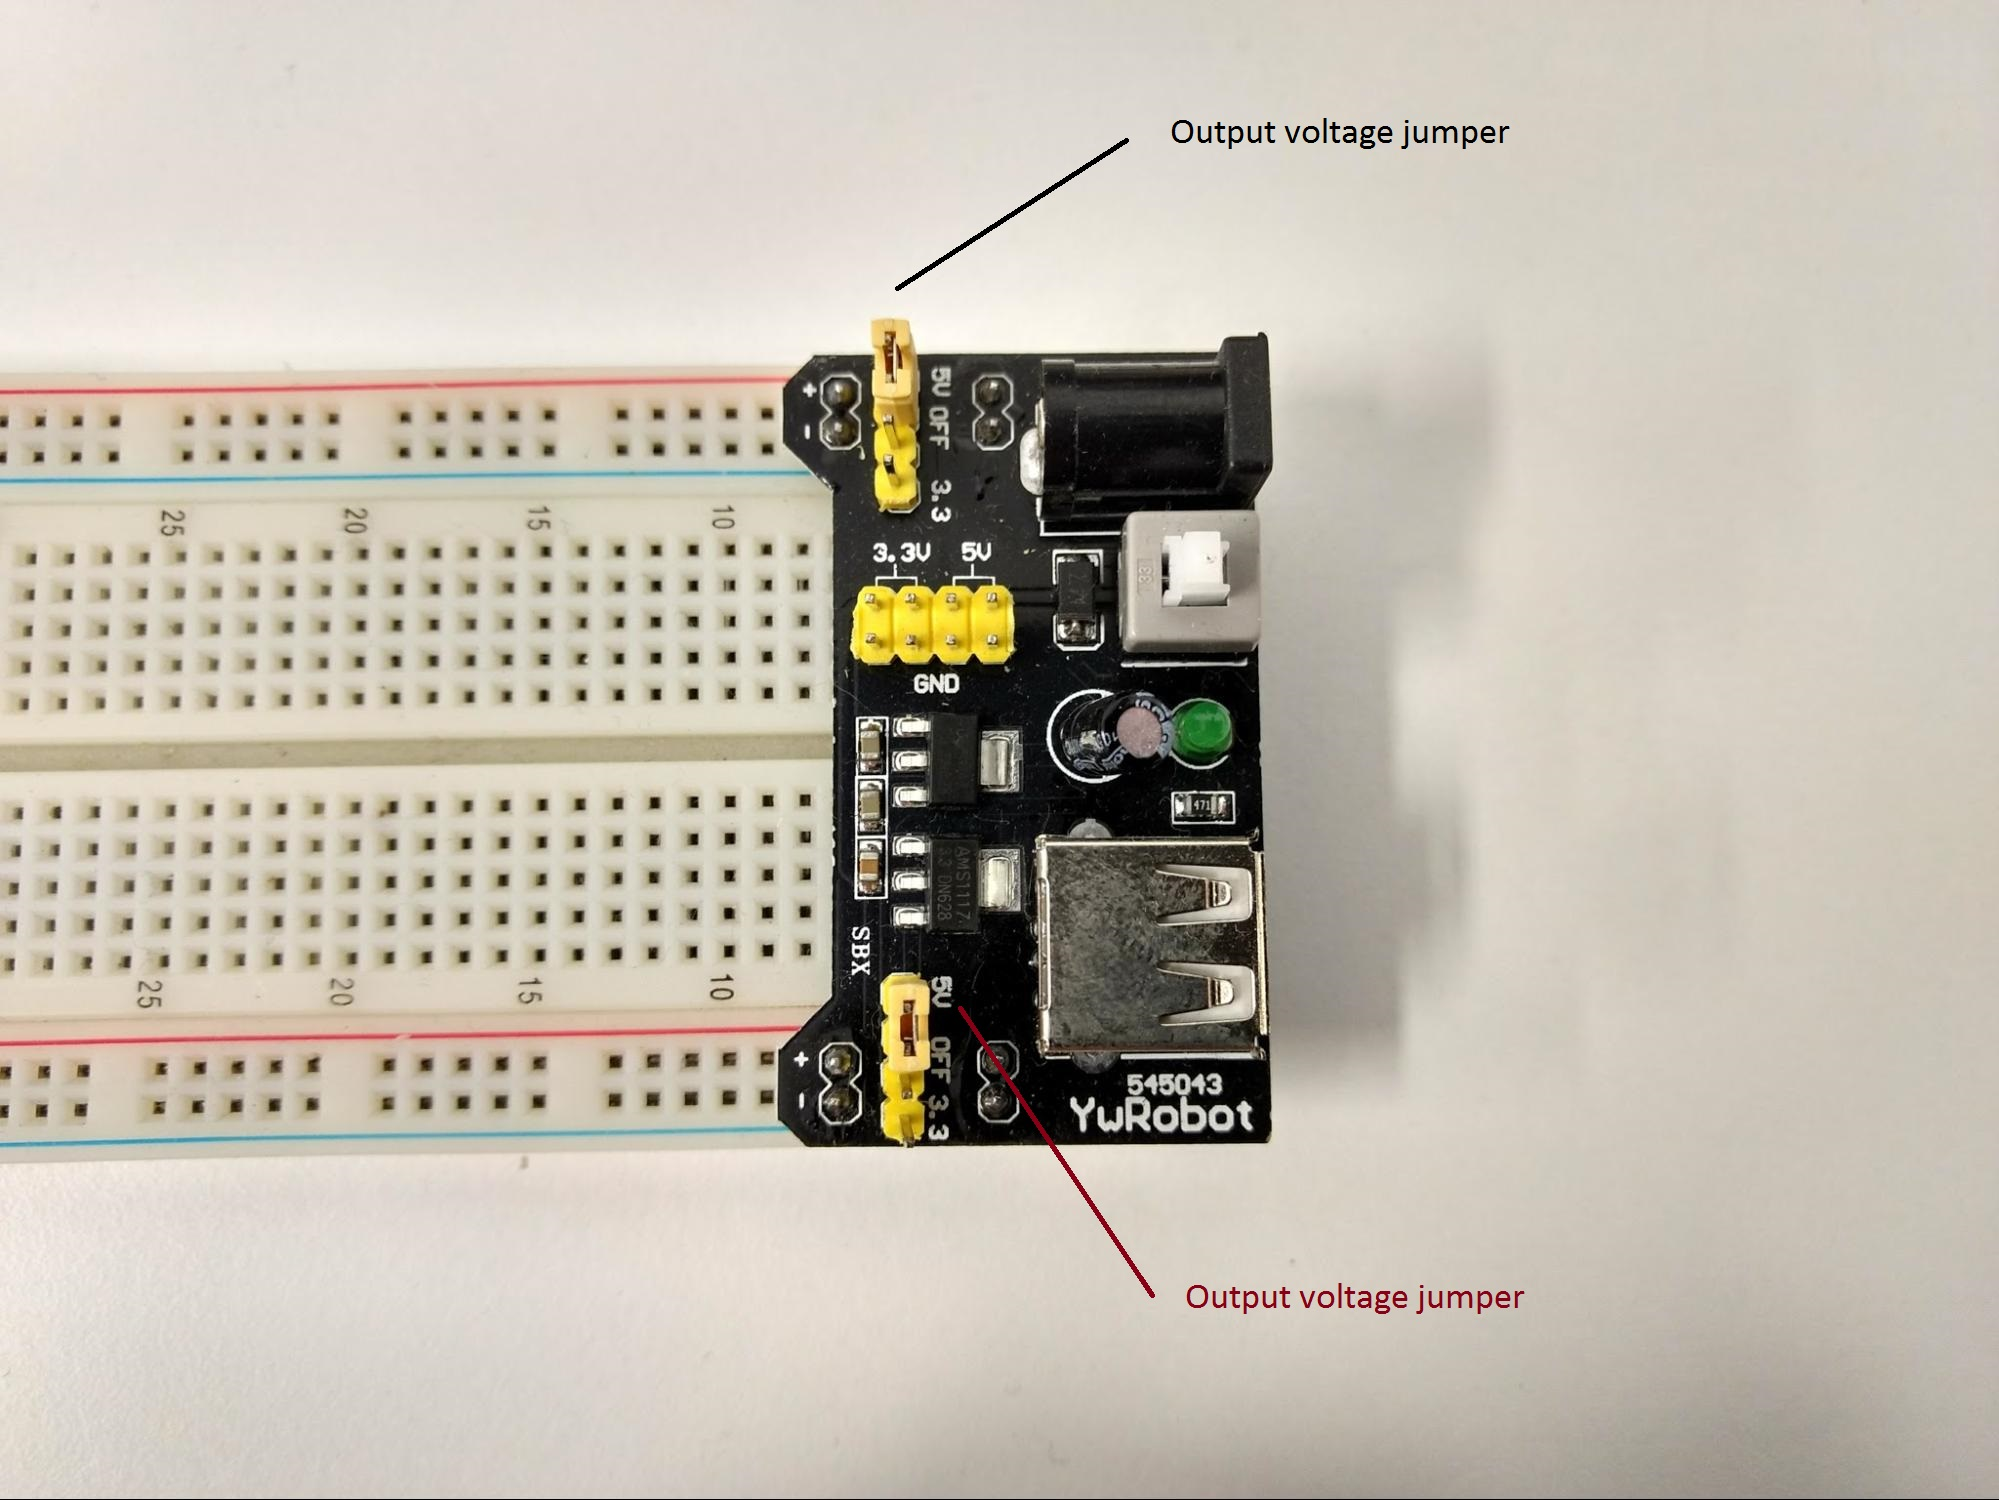
\includegraphics[width=0.6\textwidth]{Figures/bbpsu}}
    \caption{Breadboard power supply mounting}
    \label{fig:psu}
    \end{figure}
    
    
    \item Set the output voltage jumpers to +5 V, as shown in Figure \ref{fig:psu}. \\ \\ \textbf{NB:} Always double check the output voltage. In later labs involving the STM32 microcontroller +3.3 V may be used instead.

    \item Construct the circuit in Figure \ref{fig:ledcct}. The push button's pinout is shown in Figures \ref{fig:swcad} and \ref{fig:swpinout}. Use your knowledge of the breadboard's internal structure (see the knowledge reference 4.1) to make an informed choice regarding where to insert each component. Use the supplied male-male jumper wires as necessary. \footnote{See Appendix A if you need help, but try to figure it out for yourself first.}
     \item Connect the mains `plug pack' power supply to the 2.1mm DC jack on the PSU and switch on the power.
    \item Press the push button and observe the LED illuminate. When finished, switch off the power supply.

\end{enumerate}


\begin{figure}[H]
\makebox[\textwidth][c]{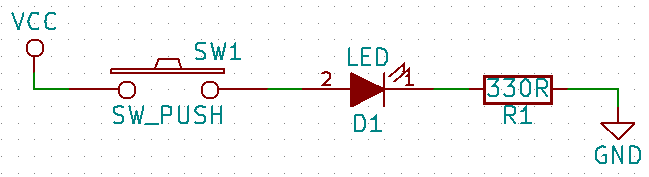
\includegraphics[width=0.7\textwidth]{Figures/LEDsch}}
\caption{LED circuit}
\label{fig:ledcct}
\end{figure}
    

\begin{figure}[H]
\makebox[\textwidth][c]{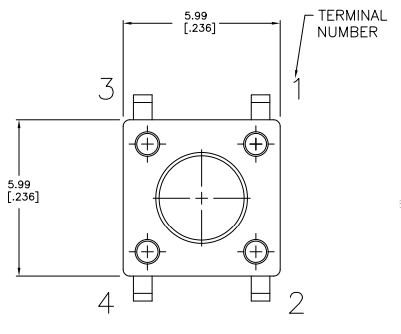
\includegraphics[width=0.5\textwidth]{Figures/swcad}}
\caption{Push button pinout}
\label{fig:swcad}
\end{figure}

\begin{figure}[H]
\makebox[\textwidth][c]{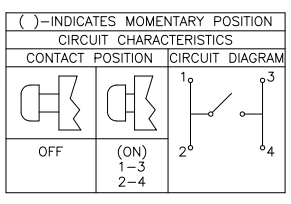
\includegraphics[width=0.5\textwidth]{Figures/swpinout}}
\caption{Push button internal connections. When the switch is 'off', pin1 is connected to pin 2 and pin 3 is connected to pin 4. When the switch is 'on' (pressed) all four pins are connected. Thus if you connect Vcc to pin 1 you can connect the LED to pins 3 or 4. }
\label{fig:swpinout}
\end{figure}

\pagebreak

\section{Using a switch as a logic source}

\begin{enumerate}
    \item Construct the circuit shown in Figure \ref{fig:swsch}.
    
    \begin{figure}[H]
    \makebox[\textwidth][c]{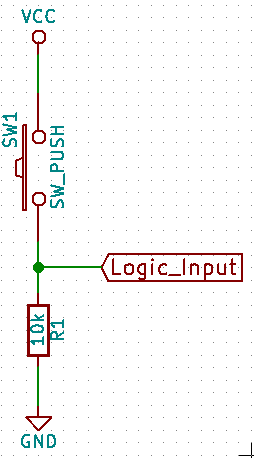
\includegraphics[width=0.23\textwidth]{Figures/swsch}}
    \caption{A basic single-pole-single-throw (SPST) switch based logic source. The 10k$\Omega$ `pull-down' resistor is required to ensure that the logic output is never `floating' (disconnected)}
    \label{fig:swsch}
    \end{figure}
    
    \item  Connect a `ground' (solid black wire) from the Saleae analyser to a `GND' pin on the breadboard. Watch the Salea introduction video if you are not sure how to do this.
    
    \item Connect channel 0 of the Saleae analyser to the node labeled \texttt{Logic\_Input} in Figure \ref{fig:swsch}. 
    
    \item Find and open the program `Logic' on the lab PC. Click the arrow next to the green button in the top left and configure the capture settings as per Figure \ref{fig:logicsettings}.
    
    \begin{figure}[H]
    \makebox[\textwidth][c]{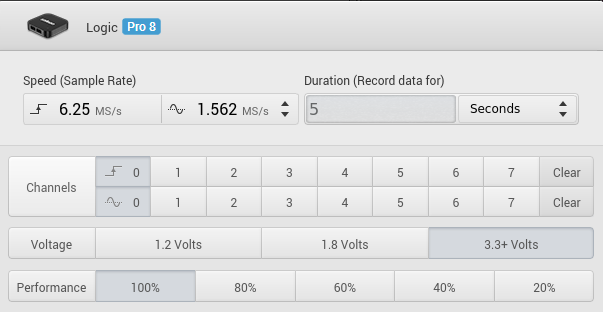
\includegraphics[width=0.7\textwidth]{Figures/logicSettings}}
    \caption{Saleae logic analyser sample rate configuration and channel selection}
    \label{fig:logicsettings}
    \end{figure}
    
    \item Click `Start' to initiate a capture while repeatedly pressing the push button. You can set the `trigger' in Logic so that it waits for a logic transition before storing a capture. The trigger control button is highlighted with a red circle in Figure \ref{fig:swbounce}
    
    \begin{figure}[H]
    \makebox[\textwidth][c]{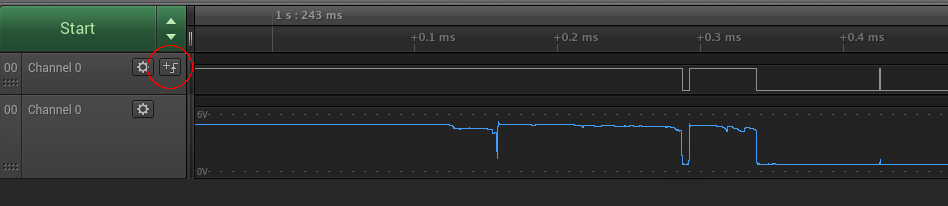
\includegraphics[width=0.8\textwidth]{Figures/swbounce}}
    \caption{A switch transition showing strong switch bounce. The red circle shows the location of the `trigger' control.}
    \label{fig:swbounce}
    \end{figure}
    
    \item Zoom in on a transition using the mouse scroll wheel. Observe that the transition between logic states is not clean but rather contains several 1/0/1/0 transitions. \textbf{NB:} Switch bounce is quite random, it may occur every transition or only every 50th. The switches are very cheap and their bounce characteristics vary dramatically between units.
    
    \item Construct the resistor-capacitor (RC) debouncing circuit shown in Figure \ref{fig:rcswsch}. (NB the theory behind the `RC filter' is beyond the scope of this course. You will learn all about capacitors in ELEC1310.)
    
    \item Perform another data capture with the logic analyser and observe the behaviour of the debounced circuit. You should be able to clearly see the smooth rise and fall of the output voltage in the analogue capture data.
    
    \begin{figure}[H]
    \makebox[\textwidth][c]{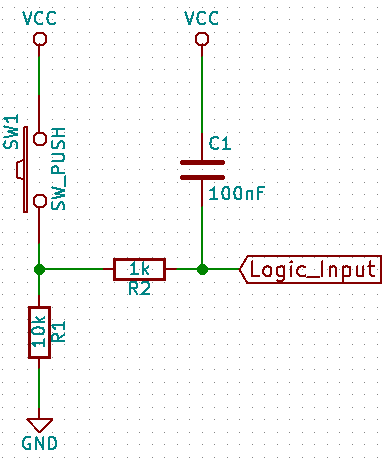
\includegraphics[width=0.4\textwidth]{Figures/rcswsch}}
    \caption{The addition of a 1k$\Omega$ resistor and 100nF capacitor is one method to minimise switch bounce seen by digital logic circuits.}
    \label{fig:rcswsch}
    \end{figure}
\end{enumerate}


Appendix A  -  Detailed instructions for Circuit 1. 

Insert the switch so that pins 1 and 3 are one one side of the breadboard horizontal mid line and pins 2 and 4 are on the other side. Chose which pair (1,3 or 2,4) you will use for your switch and connect one of the pair to Vcc (the other pin of the pair will connect to the LED).  Insert the LED and bend the legs so that the negative (cathode, short leg) is inserted into a free spot in the breadboard and the positive leg is connected to the free switch pin. Connect the resistor between the LED cathod and ground.


\end{document}